% The mrm model after Chapter 5: a reading guide for Kenny.
% Build: cd ~/mrm-model/docs/guide && tectonic mrm_guide.tex
\documentclass[11pt,letterpaper]{article}
\usepackage[margin=0.6in,top=0.6in,bottom=0.7in]{geometry}
\usepackage[compact]{titlesec}
\titlespacing*{\subsection}{0pt}{1.6ex plus .5ex}{0.6ex}
\titlespacing*{\section}{0pt}{2.2ex plus .5ex}{1ex}
\usepackage{amsmath,amssymb}
\usepackage{booktabs,tabularx,xltabular,array}
\usepackage[table]{xcolor}
\usepackage{enumitem}
\usepackage{listings}
\usepackage{xurl}
\usepackage{float}
\usepackage[colorlinks=true,linkcolor=blue!50!black,urlcolor=blue!50!black]{hyperref}
\usepackage{tikz}
\usetikzlibrary{arrows.meta,calc}

\setlength{\parindent}{0pt}
\setlength{\parskip}{2pt}
\setlist{nosep,leftmargin=1.4em}
\renewcommand{\arraystretch}{1.1}
\setlength{\abovedisplayskip}{5pt}\setlength{\belowdisplayskip}{5pt}
\setlength{\abovedisplayshortskip}{3pt}\setlength{\belowdisplayshortskip}{3pt}

% units
\newcommand{\us}{\,\ensuremath{\mu}s}
\newcommand{\um}{\,\ensuremath{\mu}m}
\newcommand{\uA}{\,\ensuremath{\mu}A}
\newcommand{\uW}{\,\ensuremath{\mu}W}
\newcommand{\degC}{\,\ensuremath{^\circ}C}
\newcommand{\cd}[1]{\path{#1}}
\newcolumntype{R}{>{\raggedright\arraybackslash}X}
\newcolumntype{P}[1]{>{\raggedright\arraybackslash}p{#1}}

% the trailer of each bridge subsection
\newcommand{\trail}[3]{%
  \par\vspace{2pt}{\small
  \begin{tabularx}{\linewidth}{@{}>{\bfseries}l R@{}}
  Code & #1\\
  g26 & #2\\
  \rowcolor{orange!10} Book & #3\\
  \end{tabularx}}\par}
\newcommand{\hard}[1]{\par\textbf{Hard point.} #1\par}
\newcommand{\grp}[1]{\multicolumn{4}{@{}l}{\rule{0pt}{2.6ex}\textbf{#1}}\\*}

\lstset{basicstyle=\ttfamily\scriptsize,breaklines=true,columns=fullflexible,keepspaces=true,
  frame=single,framerule=0.3pt,rulecolor=\color{gray},
  postbreak=\mbox{\textcolor{gray}{$\hookrightarrow$}\space}}

\begin{document}

\begin{center}
{\LARGE\bfseries The mrm model after Chapter 5}\\[3pt]
{\large A reading guide: where things are, and what the code computes}\\[4pt]
{\small For Kenny Guo. 19 October 2026. Model at commit \texttt{f3a8629} (\texttt{\textasciitilde/mrm-model}).}
\end{center}

\section*{How to use this guide}

You know textbook chapters 0 to 5. This guide connects that knowledge to the rest of the physics, and shows where
that physics is in the code. Section~1 shows the model on one page. Section~2 lists the core code in reading order.
Section~3 is the bridge, one short part per concept. Section~4 lists what remains and the first commands.

\textbf{Numbers.} Every number comes from the model preset \texttt{g26} at commit \texttt{f3a8629}
(\cd{mrm/params/presets/g26.yaml} and \cd{docs/PARAMETERS.md}). The textbook's numbers are not verified. A row
``Book'' tells you where the textbook uses another value or another method. Do not use a textbook value as a design
value. The words ``my arithmetic'' mark a number that I calculated from model values. No model output states it.

\fbox{\parbox{\dimexpr\linewidth-2\fboxsep-2\fboxrule}{\textbf{Sign convention (read this first).}
The model detuning is $d=\lambda_{res}-\lambda_{line}=-\delta$, with $\delta=\lambda_L-\lambda_r$ from the end of
Ch05. A positive $d$ means that the resonance is red of its laser line. The laser then sits on the blue flank of the
resonance. This is the stable lock side in the model and in the book. Two sign conventions are in use, so always say
where the resonance is relative to the laser. The code writes $i$ for your $j$: time dependence $e^{+i\omega t}$, and
one round trip multiplies a field by $a\,e^{-i\phi}$. This is your Ch05 convention.}}

%=====================================================================================================================
\section{The model on one page}

\textbf{What it is.} The model simulates the device that your lock controller will drive: the transmit bank of
Lightmatter's G26 link. Eight microring modulators sit on one bus waveguide. Each ring has a heater inside it, a PN
junction for the data, and a monitor photodiode (PD) on its drop port. Eight laser lines sit on a 400\,GHz grid near
1310\,nm, with 50\,Gb/s NRZ data. The plant steps in ticks of 1\us. Your controller runs every 10 ticks (100\,kHz). It
reads ADC codes and writes heater DAC codes, as firmware does.

\textbf{Why one tick can solve the optics in steady state.} The photon lifetime is $\tau_p=Q\lambda/(2\pi c)\approx
2.7$\,ps (your 5.26, with $Q=3850$). Heat moves in microseconds to milliseconds. So each tick computes the ring in
steady state at the present temperature, and a thermal network carries the slow state from tick to tick.



\textbf{How to find things.} Run these from \texttt{\textasciitilde/mrm-model}:
\begin{lstlisting}
.venv/bin/mrm params explain g26 <key>    # one number: value, source, worlds, textbook value ("disagrees:")
                                          # <key>: a leaf (ring.thermal.tau_fast_s) or a diagnostic (fwhm_pm)
grep -n "^def \|^class " mrm/plant/optics.py            # function map of a module (read its docstring first)
grep -n "q_loaded" mrm/params/r*.py                     # where a leaf enters the plant (grep the last part of its key)
grep -n "# ---" mrm/sim/kernel.py                       # sections of the compiled tick
grep -n "textbook\|disagrees" mrm/params/presets/g26.yaml   # where the model departs from the book
grep -rn "07 P0-1" mrm docs                             # follow a tag of docs/research/07_design_critique.md
\end{lstlisting}
For each plant module, \cd{tests/verification/test_<module>.py} shows its functions in use. Read first: \cd{docs/EXPLAINED.md}
(written for you), \cd{docs/ENGINE.md} sections 3--6, \cd{docs/ARCHITECTURE.md} section 2 (its note ``EXPLAINED.md
not written yet'' is stale), \cd{docs/KNOWN_ISSUES.md}. \cd{docs/PARAMETERS.md} has the derived table (line 201),
the diagnostics (line 237) and the textbook comparison (line 569). Stale: \texttt{g26\_calibrated}, both
\cd{docs/VALIDATION*.md} reports, the old A4 pass, the \texttt{InterimRom} defaults (not g26), and the header comment
of \cd{experiments/examples/a1_pi_lock.yaml} (350\,pm, now 454--473\,pm).

\textbf{Where things are.}
{\small
\begin{xltabular}{\linewidth}{@{}P{4.2cm} R@{}}
\toprule
\cd{mrm/params/} & Presets (\cd{presets/g26.yaml}), the loader, the relations R1--R5, \cd{realize.py} (draws the worlds and makes the frozen \texttt{PlantParams}).\\
\cd{mrm/plant/} & The physics of one tick: \cd{phase.py}, \cd{optics.py}, \cd{selfheat.py}, \cd{thermal.py}, \cd{electrical.py}, \cd{sensing.py}, \cd{laser.py}, \cd{datapath.py}.\\
\cd{mrm/scenarios/} & The disturbances (A1/A2 aggressor, soak, laser drift, traffic, faults) and the aggressor calibration.\\
\cd{mrm/control/} & The controller API, the knowledge tokens, and \cd{baselines/} (\texttt{pi\_lock}, dither, \texttt{wdm\_supervisor}, \ldots).\\
\cd{mrm/sim/} & The compiled tick (\cd{kernel.py}), its NumPy twin (\cd{kernel_ref.py}), the runner, the metrics, the experiments, the CLI.\\
\cd{mrm/validation/} & Published targets, the oracle, the validation report (the report is stale).\\
\cd{experiments/}, \cd{examples/} & Experiment files (\cd{examples/}, \cd{acceptance/}). Controller templates and \cd{tutorial.ipynb}.\\
\cd{docs/} & \cd{EXPLAINED.md}, \cd{ENGINE.md}, \cd{ARCHITECTURE.md}, \cd{PARAMETERS.md}, \cd{KNOWN_ISSUES.md}, \cd{handoff/} (one design note per module), \cd{research/}.\\
\cd{runs/} & One folder per run: \cd{report.txt}, \cd{metrics.json}, \cd{trace.h5}, \cd{experiment.resolved.yaml}.\\
\cd{tools/}, \cd{webviz/} & \cd{memguard.py} (stops a job above 3\,GB), \cd{clear_numba_cache.py}. A 3-D and 2-D viewer of the plant.\\
\bottomrule
\end{xltabular}}

\begin{figure}[H]
\centering
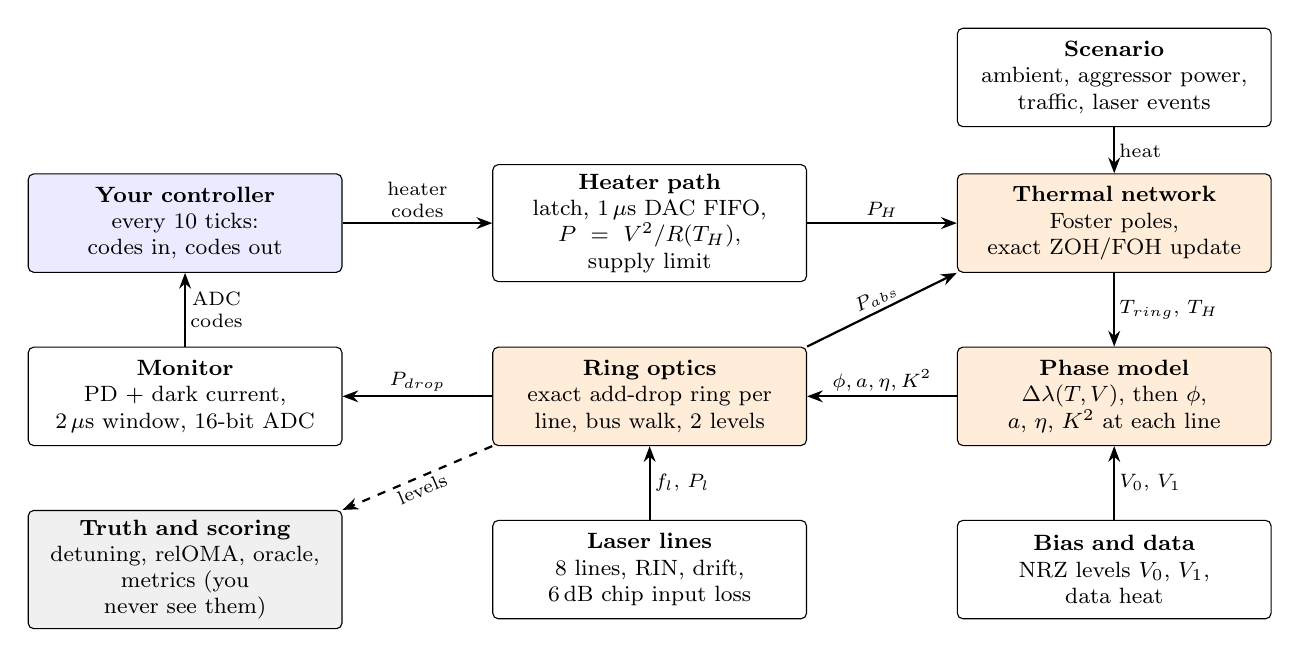
\begin{tikzpicture}[
  blk/.style={draw, rounded corners=2pt, align=center, font=\footnotesize, text width=3.75cm,
              minimum height=1.25cm, fill=#1},
  blk/.default=white,
  arr/.style={-{Stealth[length=2mm]}, thick},
  lab/.style={font=\scriptsize, inner sep=1.5pt, align=center}]
\node[blk=blue!8]    (ctrl)  at (0,0)       {\textbf{Your controller}\\every 10 ticks:\\codes in, codes out};
\node[blk]           (heat)  at (5.9,0)     {\textbf{Heater path}\\latch, 1\us{} DAC FIFO,\\$P=V^2/R(T_H)$, supply limit};
\node[blk=orange!15] (therm) at (11.8,0)    {\textbf{Thermal network}\\Foster poles,\\exact ZOH/FOH update};
\node[blk]           (scen)  at (11.8,1.85) {\textbf{Scenario}\\ambient, aggressor power,\\traffic, laser events};
\node[blk]           (mon)   at (0,-2.2)    {\textbf{Monitor}\\PD + dark current,\\2\us{} window, 16-bit ADC};
\node[blk=orange!15] (opt)   at (5.9,-2.2)  {\textbf{Ring optics}\\exact add-drop ring per\\line, bus walk, 2 levels};
\node[blk=orange!15] (ph)    at (11.8,-2.2) {\textbf{Phase model}\\$\Delta\lambda(T,V)$, then $\phi$,\\$a$, $\eta$, $K^2$ at each line};
\node[blk=gray!12]   (truth) at (0,-4.4)    {\textbf{Truth and scoring}\\detuning, relOMA, oracle,\\metrics (you never see them)};
\node[blk]           (las)   at (5.9,-4.4)  {\textbf{Laser lines}\\8 lines, RIN, drift,\\6\,dB chip input loss};
\node[blk]           (bias)  at (11.8,-4.4) {\textbf{Bias and data}\\NRZ levels $V_0$, $V_1$,\\data heat};
\draw[arr] (ctrl) -- node[lab,above]{heater\\codes} (heat);
\draw[arr] (heat) -- node[lab,above]{$P_H$} (therm);
\draw[arr] (scen) -- node[lab,right]{heat} (therm);
\draw[arr] (therm) -- node[lab,right]{$T_{ring}$, $T_H$} (ph);
\draw[arr] (bias) -- node[lab,right]{$V_0$, $V_1$} (ph);
\draw[arr] (ph) -- node[lab,above]{$\phi,a,\eta,K^2$} (opt);
\draw[arr] (opt.north east) -- node[lab,above,sloped]{$P_{abs}$} (therm.south west);
\draw[arr] (las) -- node[lab,right]{$f_l$, $P_l$} (opt);
\draw[arr] (opt) -- node[lab,above]{$P_{drop}$} (mon);
\draw[arr] (mon) -- node[lab,right]{ADC\\codes} (ctrl);
\draw[arr,dashed] (opt.south west) -- node[lab,below,sloped]{levels} (truth.north east);
\end{tikzpicture}
\caption{The signal flow of one tick. The orange blocks are solved together inside each tick (implicit
self-heating). For each ring in bus order, a Newton solve finds the temperature at which absorbed power and heat
agree. The PD temperature also goes to the monitor (not drawn). Code order per tick: edge, latch, scenario,
laser, NRZ levels, phase model (previous temperature), heater, thermal and self-heating step, monitor, Truth, metrics.}
\end{figure}



%=====================================================================================================================
\section{Core lines of code to read, in order}

Line numbers are for commit \texttt{f3a8629}. Read the docstrings first. Skip \cd{mrm/sim/kernel.py} until you need
it. It calls the leaf modules, and it copies the self-heating step line for line. \cd{kernel_ref.py} is the readable
version of the same tick.

{\footnotesize
\begin{xltabular}{\linewidth}{@{}r P{6.2cm} P{2.0cm} R@{}}
\toprule
\# & File and symbol & Lines & What to take from it\\\midrule
\endfirsthead
\toprule
\# & File and symbol & Lines & What to take from it\\\midrule
\endhead
\bottomrule
\endfoot
\grp{A. Your side of the interface (start here, to know the goal)}
1 & \cd{examples/controllers/template_python_controller.py} \cd{MyIntegralLock} & 26--57 & The file you copy. A plain integral lock of the monitor to a fraction of a known peak code.\\
2 & \cd{mrm/control/api.py} docstring; \cd{ControllerSpec}, \cd{Observation} & 1--41; 145--481, 573--611 & What a controller sees: \texttt{reset(spec)} once, \texttt{step(obs)} at each edge, integer codes back.\\
3 & \cd{mrm/core/channels.py} \cd{V1_CHANNEL_TABLE} & 367--430 & Every channel name: \texttt{tx.heater}, \texttt{tx.monitor.samples}, \texttt{tx.heater.applied}, \texttt{temp.<name>}, \ldots\\
4 & \cd{mrm/control/baselines/pi_lock.py} docstring & 1--85 & Which side to lock on and why, the MAP--RETURN--LOCK algorithm, the PI law, the failure modes.\\
\grp{B. Optics: from your Ch05 ring to the model ring}
5 & \cd{mrm/plant/optics.py} docstring & 9--42, 91--117 & Conventions and ports (0 in, 1 through, 2 drop to the monitor, 3 add). The bus and the NRZ averaging.\\
6 & \cd{mrm/plant/optics.py} \cd{_airy_line} & 528--560 & Your eq.\ (5.30), exact: $T$, $D$, the loss fraction and their $\phi$ derivatives.\\
7 & \cd{mrm/plant/phase.py} docstring, equations 1--6 & 10--64 & The phase model on one page: shift, phase at the line, group delay, $K^2$ at the line, loss and $\eta$, bus segments.\\
8 & \cd{mrm/plant/phase.py} \cd{thermal_shift_m}, \cd{resonance_shift_ws}, \cd{_fill_level} & 203--206, 229--238, 248--275 & The same equations as code: the shift per ring, then $\phi$, $a$, $\eta$, $T_{rt}$ per line.\\
9 & \cd{mrm/params/relations.py} docstring R3, R4 & 13--21, 35--47 & FSR and order from the geometry. Q values and the loss budget converted to $K_t^2$, $K_d^2$, $a$.\\
10 & \cd{mrm/plant/optics.py} \cd{ring_lines_nb} & 1029--1126 & One ring at all 8 lines: both NRZ levels, the ones-density average, $P_{abs}=\eta\mathcal{L}P_{in}$, sums for the monitor.\\
11 & \cd{mrm/plant/optics.py} \cd{ring_exact} & 2701--2718 & Python API. Use it in a notebook to check the line shape against Ch05.\\
\grp{C. Modulation}
12 & \cd{mrm/plant/electrical.py} \cd{depletion_shift_m}, \cd{analytic_junction_table_from_ring} & 1491--1505, 1540--1568 & The square-root depletion law, and the index and loss change of the junction.\\
13 & \cd{mrm/plant/electrical.py} \cd{nrz_levels_row} & 649--684 & The two junction voltages from the bias and the swing.\\
14 & \cd{mrm/sim/kernel.py} \cd{_truth_a} (relOMA lines) & 1328--1334 & relOMA $=|P_{thru,1}-P_{thru,0}|/P_{in}$ at the ring's own through port.\\
\grp{D. Heat: self-heating, thermal network, heater}
15 & \cd{mrm/plant/selfheat.py} docstring & 1--42 & The implicit per-ring solve, branch continuation, the start protocols.\\
16 & \cd{mrm/plant/selfheat.py} \cd{solve_ring_temperature} & 73--162 & Newton from the previous root. It never skips a root and follows the branch.\\
17 & \cd{mrm/plant/selfheat.py} \cd{lorentzian_folds}, \cd{bistability_ratio} & 463--489 & The analytic fold points and the bistability ratio for one line.\\
18 & \cd{mrm/plant/thermal.py} docstring; \cd{foh_scalar} & 1--55; 140--162 & Foster sums, one lag per (observer, source, pole), the exact hold update.\\
19 & \cd{mrm/plant/thermal.py} \cd{InterimRom} (docstring) & 737--781 & $Z_{RH}$, $Z_{RR}$, $Z_{HH}$ and the crosstalk rules. Its defaults are not g26.\\
20 & \cd{mrm/plant/thermal.py} \cd{crosstalk_tau_s}, \cd{site_fraction} & 823--862 & The crosstalk pole against distance. The static coupling of PDs, sensors and the aggressor.\\
21 & \cd{mrm/plant/electrical.py} docstring; \cd{heater_power_row}; \cd{supply_limit_row} & 1--43; 374--479; 482--509 & Code to heater power: DAC, driver law with TCR solved in the tick, array supply limit.\\
\grp{E. Monitor}
22 & \cd{mrm/plant/sensing.py} docstring & 1--68 & The signal chain from drop power to ADC code, and the exact noise per sample.\\
23 & \cd{mrm/plant/sensing.py} \cd{monitor_tick_row} & 291--416 & Per tick: integrate the current, take a code every 4 ticks, push it with its release tick.\\
24 & \cd{mrm/control/baselines/pi_lock.py} \cd{monitor_block_mean}, \cd{block_inputs} & 273--293 & How a controller averages the samples released since its last step.\\
\grp{F. The engine}
25 & \cd{mrm/core/timing.py} docstring & 1--61 & Integer ticks, one owner per delay, the order of events at a controller edge.\\
26 & \cd{mrm/sim/kernel_ref.py} \cd{ReferenceEngine.step} & 220--402 & The readable NumPy tick. Bit-identical to the kernel. Run it line by line in a debugger.\\
27 & \cd{mrm/sim/kernel.py} \cd{_world_loop} & 1873--2365 & The compiled tick. Markers: 1894 edge, 2060 optics inputs, 2156 heater, 2221 self-heating, 2281 sensors, 2332 Truth, 2343 metrics.\\
28 & \cd{mrm/sim/runner.py} \cd{run} & 159--271 & Build the plant, warm start, controller reset, run, collect metrics and traces.\\
\grp{G. Scoring, scenarios and parameters}
29 & \cd{mrm/validation/oracle.py} docstring & 1--46 & The OMA-optimal stable target, the oracle, and the OMA penalty.\\
30 & \cd{mrm/sim/metrics.py} docstring; \cd{summarize} & 1--55; 680--755 & Lock error, lock state, excursions, relOMA, wrong line. The summary columns.\\
31 & \cd{mrm/sim/experiment.py} \cd{_execute} (self-reference pre-run) & 1429--1452 & How the example files judge the lock about each ring's own operating point.\\
32 & \cd{mrm/scenarios/library.py} \cd{a1_slide10_aggressor} & 139--189 & The A1 trajectory, the site, and the referencing choice.\\
33 & \cd{mrm/scenarios/calibrate.py} docstring & 1--38 & How the aggressor power is solved so that ring 0 follows the target.\\
34 & \cd{mrm/params/presets/g26.yaml} sections & 233--1481 & fidelity 233, laser 279, ring 338 (optics 417, thermal 649, heater 877, junction 971, monitor 1002), controller\_interface 1143, metrics 1161, uncertainty 1168, variation 1447.\\
35 & \cd{mrm/params/realize.py} docstring; \cd{realize} & 1--28; 715--1119 & Worlds, devices, SI conversion, relations, thermal assembly, latencies in ticks.\\
36 & \cd{experiments/examples/steady_pi_lock.yaml}, \cd{a1_pi_lock.yaml} & whole files & An experiment file: preset, controller, scenario, start state, scoring.\\
\end{xltabular}}

%=====================================================================================================================
\section{The bridge: from your ring to the whole model}

\subsection{The model ring is your add-drop ring}
The model uses your add-drop equations (5.30) exactly, without the Lorentzian approximation. For each ring and each of
the 8 lines, \cd{_airy_line} computes the through power $T$, the drop power $D$ and the intrinsic-loss fraction
$\mathcal{L}$, per watt of input:
\begin{gather*}
t_j=\sqrt{1-K_j^2},\qquad k_j=\sqrt{K_j^2},\qquad a=e^{-\alpha_i L/2},\qquad
\mathcal{D}(\phi)=1-2t_1t_2a\cos\phi+(t_1t_2a)^2,\\
T(\phi)=\frac{t_1^2-2t_1t_2a\cos\phi+t_2^2a^2}{\mathcal{D}(\phi)},\qquad D(\phi)=\frac{k_1^2k_2^2\,a}{\mathcal{D}(\phi)},\\
\mathcal{L}(\phi)=\frac{k_1^2}{\mathcal{D}(\phi)}\,(1-a)\,(1+t_2^2a),\qquad P_{abs}=\eta\,\mathcal{L}\,P_{in}.
\end{gather*}
The cosine makes each formula periodic in $\phi$, so one evaluation includes every resonance order. The loss term
$\mathcal{L}$ is new to you. The factor $k_1^2/\mathcal{D}$ is the power that circulates just after the input coupler
(your build-up factor 5.27, with $ta\to t_1t_2a$). The factor $1-a$ is the power fraction lost in one half of the
ring. The factor $t_2^2a$ is the power that continues into the second half, after the drop coupler. Only the
fraction $\eta$ of that loss is absorption that heats the ring.

The preset does not give $t_1$, $t_2$ and $a$. It gives the loaded Q, the drop share $\kappa_d/\kappa$ and a loss
budget. \cd{relations.py} (R4) converts them with the exact energy decay over one round trip of duration $T_{rt}$.
This is your (5.24) with a third loss channel, the drop coupler:
\[
K_j^2=1-\exp(-\omega T_{rt}/Q_j),\quad a=\exp\!\left(-\frac{\omega T_{rt}}{2Q_i}\right),\quad
\frac1{Q_L}=\frac1{Q_i}+\frac1{Q_t}+\frac1{Q_d},\quad Q_d=\frac{Q_L}{\kappa_d/\kappa}.
\]

{\small
\begin{tabularx}{\linewidth}{@{}l l l R@{}}
\toprule
Ch05 & Model & Code name & Note\\\midrule
$\kappa_1^2,\ \kappa_2^2$ & $K_t^2,\ K_d^2$ & \texttt{k2\_th}, \texttt{k2\_dr} & Power coupling per pass, taken at the LINE wavelength.\\
$a$, $\phi$ & $a$, $\phi$ & \texttt{a\_rt}, \texttt{phi} & $\phi$ is absolute: about $2\pi\times79$ at resonance. Coupler phase $\psi=0$.\\
$n_gL/c$ & $T_{rt}=1/\mathrm{FSR}$ & \texttt{t\_rt} & Group delay of one round trip.\\
$Q$, $Q_{int}$, $Q_c$ & $Q_L$, $Q_i$, $Q_t$, $Q_d$ & \texttt{q\_loaded}, \ldots & Loaded, intrinsic, through-coupler and drop-coupler Q.\\
$\delta=\lambda_L-\lambda_r$ & $d=\lambda_{res}-\lambda_{line}$ & \texttt{detuning\_m} & $d=-\delta$. Half width $w=\Delta\lambda_{FWHM}/2$ (HWHM).\\
(5.12), (5.32) & $\partial\phi/\partial\lambda_{res}$, $\Delta\lambda$ & \cd{dphi_dlamres}, \cd{resonance_shift_ws} & Same physics, opposite sign: $\partial\phi/\partial\lambda_{res}=+2\pi n_gL/\lambda^2$. \cd{kernel.py} line 341, \cd{phase.py} line 230.\\
\bottomrule
\end{tabularx}}

\hard{The drop coupler is a weak tap: $Q_L/Q_d=0.007$. So the through port acts almost like your all-pass ring. The
drop port takes about 1\,\% of the input at the peak. To see this, put a small $\kappa_2$ into (5.31):
$T_{drop,max}$ stays small and the linewidth hardly changes. With the g26 values below, (5.31) gives a linewidth of
about 340\,pm and a drop peak of about 1.3\,\% (my arithmetic).}

\trail{\cd{optics.py} \cd{_airy_line} 528--560, \cd{ring_lines_nb} 1029--1126; \cd{relations.py} 35--47. A TCMT
form (\texttt{fidelity.optics\_model: tcmt}, a sum over the 3 nearest orders) exists. g26 does not use it.}
{$Q_L=3850$, $Q_i$ 7451--7543, $Q_t$ 7978--8084, $Q_d=5.5\times10^5$, $K_t^2$ 0.0940--0.0963, $K_d^2$
0.00145--0.00147, $a=0.94784$, $\eta=0.848$, FWHM 336--341\,pm, $L=42.27\um$ ($R=6.727\um$), $n_g=3.94$,
$T_{rt}=0.5556$\,ps. Under-coupled at the cold resonance: $t_1\approx0.952>t_2a\approx0.947$. The G25 device shows a
27.9\,dB notch at 0\,V.}
{Q 3500, FWHM 374\,pm, $n_g$ 4.2, $R$ 6.3\um. The model uses 3850, the middle of 3500--4200.}

\subsection{Where the resonance is: the phase model}
Your master formula (5.32) says that a resonance moves by $(\lambda/n_g)\Delta n_{eff}$. The model computes this shift
once per ring and tick, from the ring temperature $T$ and the junction voltage $V$ (\cd{phase.py} equation 1):
\[
\Delta\lambda(T,V)=s_0\Big[(T-T_{ref})+\tfrac{\beta}{2}\big((T-T_0)^2-(T_{ref}-T_0)^2\big)\Big]+\frac{\lambda_{res}}{n_g}\Big[f\,\Delta n_{eff}(V)-f\,\Delta n_{eff}(V_{ref})\Big].
\]
The first term is the heat (section~\ref{sec:to}). The second term is the junction (section~\ref{sec:mod}). Then the model moves the whole cold phase curve by that shift (a ``rigid comb''), and reads the phase at each laser
line (equation 2):
\begin{gather*}
x=\lambda_l-\Delta\lambda,\qquad \Delta=x-\lambda_{res},\qquad
n(x)=n_{eff}+(n_{eff}-n_g)\frac{\Delta}{\lambda_{res}}-\frac{n_g'\,\Delta^2}{2\lambda_{res}},\qquad \phi=\frac{2\pi\,n(x)\,L}{x}.
\end{gather*}
$\phi=2\pi m$ exactly when the shifted resonance reaches the line. Each ring is built 7.6\,nm blue of its own line,
so $\lambda_{res}^{cold}=\lambda_{line}-\Delta\lambda_{off}$. The order is $m=\mathrm{round}(n_{eff}L/\lambda_{res})$.
\cd{relations.py} (R3) then sets $n_{eff}^{ph}=m\lambda_{res}/L$, so the cold resonance sits exactly at the offset. The couplings are taken at the
line, $K_j^2(\lambda_l)=K_{j,0}^2\exp[\partial_\lambda\ln K_j^2\,(\lambda_l-\lambda_{res})]$. So under lock the notch
depth does not follow the heater code. The loss follows the junction and the temperature:
$\alpha_i=[\alpha_{i,ref}+f\alpha_{fca}(V)-f\alpha_{fca}(V_{ref})]\,e^{c_R(T-T_{ref})+c_H(T_H-T_{ref})}$ and
$\eta=\alpha_{heat}/\alpha_i$ (equation 5).

\hard{The rigid comb moves every order by the same shift, so a heated ring keeps its cold FSR in wavelength. The
locked order is exact. The adjacent orders are off by $\pm33$\,pm at the 7.6\,nm lock (KNOWN\_ISSUES item 15). This
error reaches only the foreign-line terms.}

\trail{\cd{phase.py} docstring 10--64, \cd{_fill_level} 248--275, \cd{coupling_row} 316--328; \cd{realize.py} line 1169 (cold resonance).}
{Ring 0 on 1318.6\,nm \ldots\ ring 7 on 1302.6\,nm. Cold resonances 1311.0 \ldots\ 1295.0\,nm. $m=79$ (ring 7: 80).
FSR 1.8\,THz = 10.19--10.44\,nm. $T_{ref}=25\degC$, $V_{ref}=0$\,V, $c_R=c_H=0$.}
{Keeps a measured FSR bound above 14.1\,nm. The model treats that bound as unsupported and uses the 1.8\,THz design value.}

\subsection{Modulation: the PN junction and the two data levels}\label{sec:mod}
Free carriers lower the silicon index and absorb light (the plasma-dispersion effect). A PN junction runs around a
fraction $f$ of the ring. Reverse bias widens the depletion region and removes carriers. So $n_{eff}$ rises, the
resonance moves red, and the loss falls. In an abrupt junction the depletion width, and so the removed charge, grows
as $\sqrt{V+V_{bi}}$. So the model uses a square-root law. Here $m=0.5$ is the depletion exponent, not the resonance order:
\begin{gather*}
\Delta\lambda_J(V)=A\big[(V+V_{bi})^{m}-V_{bi}^{m}\big],\qquad A=\frac{\mathrm{eff}_0\,V_{bi}^{1-m}}{m},\qquad
\frac{d\lambda}{dV}=A\,m\,(V+V_{bi})^{m-1},\\
\Delta n_{eff}(V)=\frac{n_g}{\lambda}\,\Delta\lambda_{full}(V),\qquad \alpha_{fca}(V)=\alpha_0-\frac{4\pi q}{\lambda}\,\Delta n_{eff}(V).
\end{gather*}
Here $\mathrm{eff}_0$ is the shift per volt at 0\,V, $\alpha_0$ the free-carrier loss at 0\,V, and $q=\lambda\Delta\alpha/(4\pi\Delta n)$ the
scaled ratio of loss change to index change. $\Delta\lambda_{full}=\Delta\lambda_J/f$ is the shift that a junction around the full ring
would give. The code multiplies the index and loss change by $f$ again at run time. The data swings the junction
between $V_0=V_b-V_{pp}/2$ and $V_1=V_b+V_{pp}/2$ (bias $V_b$, swing $V_{pp}$). Level 1 has the higher reverse
voltage, so it is redder and has less loss. The ring is solved at both levels every tick. Every output is the
average over the ones density $p_1$: $\bar X=p_1X(\phi_1,a_1,\eta_1)+(1-p_1)X(\phi_0,a_0,\eta_0)$.

\hard{Bias moves the ring in two ways at once. The index change moves it red. The loss change alters the absorbed
heat, and that moves it back. At the g26 lock a 0.2\,V bias step moves the resonance only 0.1--0.5\,pm, against
about 10\,pm from the index law alone. This is an open physics check. Data also heats each ring by about 2\,K
(junction charging and the driver), so traffic start, stop and squelch are thermal steps.}

\trail{\cd{electrical.py} \cd{depletion_shift_m} 1491--1505, \cd{analytic_junction_table_from_ring} 1540--1568,
\cd{nrz_levels_row} 649--684, \cd{data_activity_heat_row} 879--911. \cd{materials.py} \cd{plasma_dispersion}
680--715 is used offline only.}
{$\mathrm{eff}_0=72.5$\,pm/V at 0\,V, about 32\,pm/V at 3.75\,V. $A=137.6$\,pm/V$^{1/2}$, $V_{bi}=0.9$\,V, $f=0.8$,
$q=0.06$. Bias 1.05\,V, swing 1.3\,Vpp, so $V_0=0.40$\,V and $V_1=1.70$\,V. By the index law the two levels sit
about 65\,pm apart (my arithmetic).}
{Interpolates the G25 bias ladder up to 1.6\,V and lists a flat 50\,pm/V. Lists 0.9\,Vpp as the bench swing. The
model reads 0.9\,V as the pattern-generator swing and uses 1.3\,V. No absorbed-heat term in the bias shift.}

\subsection{OMA and relOMA}
The receiver decides between the two data levels. So the useful signal is the difference of the two through powers,
the optical modulation amplitude (OMA):
\begin{gather*}
\mathrm{relOMA}=\frac{|P_{thru,1}-P_{thru,0}|}{P_{in}},\qquad \mathrm{OMA}_{bus}=|P_{out,1}-P_{out,0}|,\\
\mathrm{BER}=\tfrac12\,\mathrm{erfc}\!\big(Q/\sqrt2\big),\qquad Q=q_{ref}\,\mathrm{OMA}_{rx}/\mathrm{OMA}_{sens}.
\end{gather*}
Here $q_{ref}$ is the Q-factor at the receiver sensitivity $\mathrm{OMA}_{sens}$. For a small level separation, the
OMA is about $P_{in}\,|dT/d\lambda|$ times the separation. So the OMA follows the slope of the notch at the operating
point, not the depth of the notch.

\hard{A deep notch (large extinction ratio) does not give a large OMA. To see this, sketch the notch and project the
two resonance positions onto it. At the notch bottom the two powers are almost equal.}

\trail{\cd{kernel.py} \cd{_truth_a} 1328--1334 (relOMA), 2276--2278 (bus OMA and BER); \cd{datapath.py} \cd{ber_from_oma} 185--193.}
{About $-6.1$\,dB at the lock (CAL-14: $-6.07$\,dB), against the printed $-2.1$\,dB. This target fails (KNOWN\_ISSUES
item 30). \cd{docs/research/07_design_critique.md} D9 notes that OMA in dBm at the actual $+4$\,dBm input would close
the gap. That reading is the open question Q4.}
{relOMA = OMA / 1\,mW at the modulator, which is that second reading. The model divides by $P_{in}$ at the ring, on
its own line (07 D9).}

\subsection{The operating point: a side-of-fringe lock}
For a Lorentzian notch, the slope $|dT/d\lambda|$ is largest at a distance $\mathrm{FWHM}/(2\sqrt3)$ from the
resonance, about 0.29 FWHM. The OMA is largest there. Near that point the OMA loss grows as the square of the lock
error. The monitor also gives a signed error on one flank. So the lock point is a set-point on a flank, not the
resonance. \texttt{pi\_lock} sets its target at a fraction $f$ of the measured drop peak. For a pure Lorentzian
that puts the ring at
\[
d_{set}\approx w\sqrt{1/f-1}\qquad(w=\mathrm{HWHM}).
\]
The oracle (section~\ref{sec:score}) finds the exact optimum with the exact ring, the bus, both levels and self-heating.

\hard{Both flanks give almost the same OMA: the best point on the blue side has 92--94\,\% of the best OMA. Only the
red side ($d>0$) is stable with self-heating (sections~\ref{sec:sh} and~\ref{sec:bist}). Use $\mathrm{FWHM}/(2\sqrt3)$ as the first
estimate and the oracle as the exact answer.}

\trail{\cd{oracle.py} docstring 13--22; \cd{pi_lock.py} docstring ``Which side, and why'' 8--22.}
{Oracle optimum $d=+103$ to $+105$\,pm. $\mathrm{FWHM}/(2\sqrt3)\approx98$\,pm (my arithmetic). \texttt{pi\_lock}
uses $f=0.7$, so $d_{set}\approx0.65w\approx110$\,pm. The settled warm start sits at $+97$ to $+121$\,pm. The 5\,pm
lock budget is 1.5\,\% of a linewidth.}
{$\delta_{opt}=374/(2\sqrt3)\approx108$\,pm, from its unverified Q.}

\subsection{WDM: eight rings on one bus}
Eight lines share one bus, at $f_k=f_c+(k-\tfrac{L-1}{2})\Delta f$ and $\lambda_k=c/f_k$. Light meets ring 0 first.
Each ring sees the averaged through power of the rings before it, times the loss of the bus segment. Lines add as
powers, because different frequencies do not interfere:
\[
P_{in,k,l}=P_{chip,l}\;t^2_{seg,k}\prod_{j\ \text{before}\ k}t^2_{seg,j}\,\bar T_{j,l},\qquad
P_{drop,k}=\sum_{l}\bar D_{k,l}\,P_{in,k,l},\qquad P_{abs,k}=\sum_l \overline{\eta\mathcal{L}}_{k,l}\,P_{in,k,l}.
\]
Every ring absorbs and drops all 8 lines. So each monitor sees a small background from the foreign lines. In the
engine this bus walk runs inside the self-heating solve, ring by ring in bus order.

\hard{The ring comb (one FSR, about 10.3\,nm) and the line comb (2.29\,nm) have different periods. A cold ring sits
7.6\,nm blue of its own line, which is about 2 FWHM blue of line $n+3$. A heater ramp from cold crosses foreign lines.
Self-heating can capture the ring on one of them. A single-ring loop cannot see the difference. A supervisor
(\texttt{wdm\_supervisor}) assigns the lines at start-up. To see it, draw both combs and slide the ring comb red from
7.6\,nm blue.}

\trail{\cd{realize.py} \cd{line_frequencies_hz} 578--592; \cd{phase.py} \cd{bus_t2_from_plant_params} 184--200;
\cd{optics.py} docstring ``Bus'' 91--108, \cd{selfheat_commit} 1527--1557; \cd{kernel.py} wrong-line block 1348--1374.}
{Line 0 is the lowest frequency (1318.6\,nm). Ring $k$ on line $k$. Segment transmission 0.99916, so ring 7 gets
0.59\,\% less light than ring 0. $+4$\,dBm per line at ring 0 (10\,dBm at the laser module, less 6\,dB chip input
loss). The next order sits 2.8--3.0 FWHM from a line. Above about 113\degC{} ambient a ring needs one more FSR of heating.}
{Ch07 sizes the heater for a generic 4.5\,nm blue offset. It also quotes Lightmatter's measured 7.6\,nm, which the
model uses. 14\,dBm per line at the laser, against 10\,dBm. Both give $+4$\,dBm at the ring.}

\subsection{The thermo-optic shift}\label{sec:to}
Heat raises the silicon index, so the resonance moves red. Your master formula with $\partial n_{eff}/\partial T$ and
the thermal expansion $\alpha_L$ gives the slope $s=d\lambda_r/dT$. The slope grows with temperature. The ring locks
at the temperature where the integral of $s$ equals the built-in offset:
\[
s(T)=\frac{\lambda}{n_g}\Big(\frac{\partial n_{eff}}{\partial T}+n_{eff}\,\alpha_L\Big)=s_0\big[1+\beta(T-T_0)\big],\qquad
\int_{T_{ref}}^{T_{lock}}s(T)\,dT=\Delta\lambda_{off}\ (\mathrm{mod}\ \mathrm{FSR}_\lambda).
\]
Each tick, the code expands the same law about the previous ring temperature (\cd{local_thermo_optic}). The
self-heating solve then uses the exact local slope.

\trail{\cd{relations.py} R1 22--24; \cd{phase.py} \cd{thermal_shift_m} 203--206, \cd{local_thermo_optic} 209--215; \cd{optics.py} \cd{_sh_prepare} 1486--1504.}
{$s_0=65.075$\,pm/K at 25\degC, 73.89\,pm/K at the lock, $\beta=1.2377\times10^{-3}$/K. Lock at 134.38\degC{}
(about 109\,K of heating) at 25\degC{} ambient. One world uses one $s$ law for every ring. World H86 (86\,pm/K,
constant): \texttt{--alt uncertainty.thermo\_optic=H86}.}
{86\,pm/K held constant, and $dn_{Si}/dT=1.86\times10^{-4}$/K (a C-band value). The model uses its 1310\,nm solver value.}

\subsection{Self-heating: an inner feedback loop}\label{sec:sh}
The ring loses part of the circulating light, and the fraction $\eta$ of that loss heats the ring. The absorbed power
peaks near resonance, like the drop curve. Heat moves the resonance red, and that changes the absorbed power again.
Treat this as an inner proportional loop around the ring temperature. The self-heating gain $G_{sh}$ converts
absorbed power to resonance shift. $Z_0$ is the thermal resistance from the heater to its ring (K/mW). The factor $z$
says that one milliwatt of absorbed light heats the ring $z$ times more than one milliwatt of heater power. Let $u$ be
the detuning that the heater alone would give:
\[
G_{sh}=s(T)\,Z_{opt},\quad Z_{opt}=z\,Z_0;\qquad \text{stable iff } G_{sh}\,\frac{\partial P_{abs}}{\partial\lambda_{res}}<1;\qquad
\frac{dd}{du}=\frac{1}{1+G_{sh}\,|P_{abs}'|}\ \ (\text{red side}).
\]
On the red side ($d>0$), heat moves the resonance away from the laser, so $P_{abs}$ falls and opposes the heat. This
is negative feedback. The relief $1+G_{sh}|P_{abs}'|$ divides the effect of the heater and of every other
disturbance. On the blue side the feedback is positive. The code solves the loop implicitly, ring by ring in bus
order, with Newton from the previous root:
\[
F(T_k)=T_k-T_k^{other}-g_k\,P_{abs,k}(T_k)=0,\qquad g_k=\sum_j(1-a_j)\,r_j^{opt},\quad a_j=e^{-h/\tau_j}.
\]
An explicit update (with the previous tick's $P_{abs}$) oscillates with period 2 at 1\us{} steps, so the code does
not use one. A start from the previous root keeps the ring on its own branch.

\hard{The plant you control is the ring with the light on. At the g26 lock its heater gain is the dark gain divided by
3 to 7, and its response is faster. A controller tuned on the dark ring has the wrong gain.}

\trail{\cd{selfheat.py} docstring 1--42, \cd{solve_ring_temperature} 73--162, \cd{implicit_step_b} 174--289;
\cd{kernel.py} \cd{_implicit_step_eng} 902--1032 (a mirror: edit both or the parity test fails).}
{$\eta=0.848$, $z=1.76$, $G_{sh}=741.8$\,pm/mW ($=1.76\times5.704$\,K/mW$\times73.89$\,pm/K), $P_{abs,peak}\approx2.09$\,mW
per ring. At the oracle target $G_{sh}\,\partial P_{abs}/\partial\lambda_{res}=-4.7$ to $-5.4$, so the relief is 5.7 to
6.4 (my arithmetic). About 43\,\% of the optical heat arrives with a 0.4\us{} pole.}
{$\eta=0.3$ and one thermal resistance for heater and light ($z=1$), so it finds only a halving of the heater gain.
The stress world: \texttt{--alt uncertainty.self\_heating.eta=stress\_0p3}.}

\subsection{Bistability: two branches and a fold}\label{sec:bist}
When the thermal pull is strong, one heater code gives three self-consistent resonance positions. The middle one is
unstable. The outer two form a hot branch and a cold branch. A ring stays on its branch until the branch ends at a
fold, and then it jumps to the other branch. Use the normalized detuning $y=(\lambda_r-\lambda_L)/\mathrm{HWHM}$ and
the pull $A=G_{sh}\,P_{abs,peak}/\mathrm{HWHM}$:
\[
r_{bist}=\frac{G_{sh}\,P_{abs,peak}}{(4\sqrt3/9)\,\mathrm{FWHM}}>1\ \Rightarrow\ \text{bistable};\qquad
\text{folds: } (1+y^2)^2+2Ay=0.
\]
To see it, plot the self-heating shift $A/(1+y^2)$ against $y$, and draw the heater line $y-y_o$. One crossing gives
one state. Three crossings give bistability. The direction of approach picks the branch.

\hard{The drop peak looks like the best place to lock. In g26 the fold is only about 9\,pm blue of the drop peak. A
small push or probe from the peak crosses the fold. The ring then jumps about 1.5\,nm blue. The peak-seeking
controllers stop at the peak, next to the fold, at about 13\,dB OMA penalty.}

\trail{\cd{selfheat.py} \cd{lorentzian_folds} 463--478, \cd{bistability_ratio} 487--489; start protocols
\texttt{branch\_low}, \texttt{branch\_high}, \texttt{laser\_ramp} in \cd{docs/ENGINE.md} section 3.}
{$r_{bist}=5.93$--5.98 at $+4$\,dBm (\texttt{mrm params explain g26 bistability\_ratio}).}
{A much weaker pull ($\eta=0.3$, $z=1$).}

\subsection{The heater law}
A 16-bit voltage DAC drives each heater. So $P=V^2/R$, and the gain per code grows with the code. The resistance
rises with the heater temperature (TCR), and that makes the gain droop at high drive. The code solves this inside
the tick, with $T_H=t_{pre}+g_{self}P$. Here $t_{pre}$ is the heater temperature without the power of this tick, and
$g_{self}$ (K/W) is the rise that this tick's own power gives:
\begin{gather*}
u=\frac{\mathrm{code}}{2^{16}-1},\qquad V=u\,V_{FS},\qquad R=R_0\big[1+\alpha_{TCR}(T_H-T_0)\big],\\
P=\frac{2V^2}{r_o+\sqrt{r_o^2+4kV^2}},\qquad r_o=R_0\big[1+\alpha_{TCR}(t_{pre}-T_0)\big],\qquad k=R_0\,\alpha_{TCR}\,g_{self}.
\end{gather*}
With $g_{self}=R_{th,H}$ and $t_{pre}=T_0$ this is the static law $P(1+yP)=V^2/R_0$, $y=\alpha_{TCR}R_{th,H}$. All
heaters share one supply. Above its limit one droop factor scales every heater:
$s=\min(1,\sqrt{P_{max}/\sum P},\,I_{max}/\sum I)$ and $P\to s^2P$ (here $s$ is the droop factor, not the
thermo-optic slope). The tuning efficiency is $\eta_H=\mathrm{FSR}_\lambda/P_{FSR}$.

\hard{A heater can only heat. Code 0 is zero heat. If a disturbance heats the ring more than the heater's share of
the lock temperature, no controller can cancel it. This limit is ``heater authority''. For a design, linearize about
the operating code with $dP/d\mathrm{code}\approx2P/\mathrm{code}$, and schedule the gain as
$1/\mathrm{code}$ (the $\sigma(u)$ of \texttt{pi\_lock}).}

\trail{\cd{electrical.py} docstring 1--43 (actuator path), \cd{dac_frac} 119--140, \cd{heater_power_row} 374--479,
\cd{supply_limit_row} 482--509; \cd{kernel.py} 2156--2217.}
{$V_{FS}=1.6$\,V (assumed), $R_0=45.41\,\Omega$, $\alpha_{TCR}=1.4\times10^{-3}$/K, $P_{FSR}=25.45$\,mW, so
$\eta_H=0.4046$\,nm/mW and $Z_0=5.704$\,K/mW. $y=0.00904$/mW. Full scale about 41\,mW (about 1.6 FSR). Dark gain
about 0.18\,pm/code at a quarter of full scale and 0.54 at three quarters. Ring 0 uses about 14\,mW at the lock
(about 81\,K of its 109\,K). DAC latency 1\us. Supply limit 0.2\,W and 0.15\,A (assumed). It binds in about 1/3 of
the sampled worlds.}
{TCR $10^{-3}$/K on the heater's own heat only, 4.7\,K/mW. Its 19\,500--49\,300 codes are one G26 test, not the DAC range.}

\subsection{Thermal dynamics and crosstalk}
Heat flow obeys the same equations as an RC network: power is the current, temperature rise is the voltage. The model
writes every path from a heat source to an observer as a Foster sum of first-order poles. Each pole is one lag. The
code advances each lag exactly over a step $h$, for a held input (ZOH, $u_0=u_1$) or a linear one (FOH):
\[
Z(s)=\sum_k\frac{r_k}{1+s\tau_k},\qquad
x_m\leftarrow a_mx_m+r_m\big(b_0u_0+b_1u_1\big),\quad a=e^{-h/\tau},\ b_1=1-\frac{1-a}{h/\tau},\ b_0=\frac{1-a}{h/\tau}-a.
\]
The heater reaches its own ring through three poles,
$Z_{RH}(s)=Z_0\big[\frac{f_F}{1+s\tau_F}+\frac{1-f_F-f_T}{1+s\tau_S}+\frac{f_T}{1+s\tau_T}\big]$. The absorbed light
uses $Z_{RR}$, which is $z$ times larger and has an extra fast pole. Ring-to-ring crosstalk is one pole per pair,
$cZ_0/(1+s\tau_{xt}(d))$, and it is slower for a larger distance. PDs, the die sensor and the aggressor use the same
distance laws.

\hard{There is no single thermal time constant. Read the step response as a sum of exponentials, and read its Bode
phase near your crossover. The crosstalk in g26 is weak and slow, so it acts like a slow disturbance, not a fast
coupling between loops.}

\trail{\cd{thermal.py} docstring 1--55, \cd{foh_scalar} 140--162, \cd{InterimRom} 736--820,
\cd{crosstalk_tau_s} 823--851, \cd{site_fraction} 854--862, \cd{_interim_lags} 1122--1205.}
{Heater to own ring: 41\,\% at 3.18\us, 54\,\% at 13.0\us, 5\,\% at 3\,ms. Light: $1.76Z_0$, 43\,\% at 0.4\us.
Nearest neighbour 3\,\% with a 1.52\,ms pole, others 1.5\,\%. Own PD 0.38\,ms. Aggressor to ring 0: 6\,\% of $Z_0$,
0.62\,ms. Die sensor at 1\,mm: 1.5\,\%, about 9\,ms. These are imec numbers, not G26 numbers. The G26 package is
unknown: corner \texttt{g26\_tec\_package} gives 1.0\,\% nearest in 0.12\,ms.}
{10\us{} (75\,\%) + 300\us{} (25\,\%), 10\,\% and 3\,\% crosstalk at the speed of the own heater. Corner
\texttt{g26\_textbook\_thermal} runs that network.}

\subsection{The aggressor (scenario A1)}
The aggressor is an on-die heater next to ring 0. Lightmatter drives it as the design-case disturbance. The model
injects its power at a layout site, so ring 0, the other rings, the PDs and the die sensor each see it through their
own thermal path. Before the run, the code solves for the non-negative power waveform that makes ring 0 follow the
published trajectory:
\begin{gather*}
T_{A1}(t)=113.6-88.5\,\big|\sin(\pi t/P)\big|\ {}^{\circ}\mathrm{C},\qquad P=130.7\ \mathrm{ms},\qquad
\max|\dot T|=\frac{\pi\,\Delta T}{P}=2127\ \mathrm{K/s},\\
\Delta\lambda_{tgt}(t)=s_{ref}\big(T_p(t)-T_{base}\big),\qquad s_{ref}=15\ \mathrm{GHz/K}\cdot\frac{\lambda^2}{c}=85.86\ \mathrm{pm/K}.
\end{gather*}
With the default ``resonance'' referencing, the printed $^\circ$C become a resonance target. The code then applies
the model's own $s(T)$ once, to convert that target into a ring temperature rise.

\hard{The swing is about 7.6\,nm of resonance. Ring 0's heater share of its lock is about 81\,K, roughly 6\,nm. So
at the hot cusp ring 0's heater reaches code 0 and stays there for about 15\,ms, whatever the loop does. To see it,
compare the disturbance swing in pm with the heater range in pm. The remainder is about 1.6\,nm (my arithmetic). The ring
does not move by all of it. It moves red, absorbs less light and cools (section~\ref{sec:sh}). So it leaves
its point by about 0.45\,nm.}

\trail{\cd{scenarios/library.py} \cd{a1_slide10_aggressor} 139--189; \cd{scenarios/calibrate.py} docstring 1--38,
\cd{calibrate_aggressor_power} 517--629; \cd{experiments/examples/a1_pi_lock.yaml}.}
{Peak rate 2127\,K/s, mean rate 1354\,K/s. Peak target rate about 183\,pm/ms at ring 0. Site 30\um{} from ring 0 and
55\um{} from PD0 (assumed). Ring 0 leaves its point by 454--473\,pm with every controller tried (KNOWN\_ISSUES item 38). Rings 1--7 stay
within about 15\,pm (\texttt{pi\_lock}: ring 4 14.7\,pm, ring 5 6.4\,pm, the others within 2.5\,pm).}
{Injects the swing as a temperature at the ring node only, so nothing else on the die feels it. Rate $-2300$ to $+2200\degC$/s (read from a figure).}

\subsection{The monitor and the ADC: what a code means}
Each ring has a germanium PD on its drop port. The controller never sees the current. It sees 16-bit codes. The PD
current, plus a dark current that grows with the PD temperature, is integrated over a window $W$. One noise sample of
exact variance is added, and the ADC converts the mean:
\[
i_{sig}=g_s\,\mathcal{R}\,(P_{drop}+f_{bg}P_{bus}),\qquad
\bar x=\frac{1}{W}\sum_{k\in(s-W,s]}(i_{sig}+i_d)+\sigma \xi,\qquad \sigma^2=\frac{S}{2T_W},\qquad
\mathrm{LSB}=\frac{I_{FS}}{2^{16}-1}.
\]
Here $g_s$ is the monitor gain scale and $f_{bg}$ the background fraction (0 in g26). $W$ is the window in ticks
($T_W$ in seconds) and $s$ the sample tick. $S=2q(i_{sig}+i_d)+S_{TIA}$ is the one-sided noise density, with $q$ the
electron charge. $\xi$ is one draw from a unit normal distribution. The drop reading peaks at the resonance and is
even in detuning. On one known flank the level gives the direction.
On the red lock side, more heater moves the resonance further red, so the code falls ($dy/du<0$).

\hard{Noise is not the limit. Shot noise in one 2\us{} sample is about 1\,nA, about 0.01\,pm (my arithmetic).
Systematic errors dominate: the monitor gain (worlds scale it by 0.5--2), the dark current, and light from foreign
lines. An extra current $\Delta i$ moves a level lock by $\Delta i$ divided by the monitor slope. So the shipped locks
normalize to a peak that they measure.}

\trail{\cd{sensing.py} docstring 1--68, \cd{dark_current_a} 194--203, \cd{adc_quantize} 222--257,
\cd{monitor_tick_row} 291--416; \cd{pi_lock.py} \cd{block_inputs} 285--293.}
{$\mathcal{R}=0.95$\,A/W, $I_{FS}=40\uA$, LSB $=0.610$\,nA (1556 codes per \uW{} of drop power). Window 2\us,
one code every 4\us{} (250\,kHz), latency 2\us. Dark current 5\,nA at 25\degC{} ($\times1.6$ per 10\,K). Drop peak
about 32\uA. The monitor current at the lock misses its target (CAL-8: 18.6 against 15.5\uA).}
{No dark current, 6.4\,pA/$\sqrt{\mathrm{Hz}}$ (model 1), 15--20\uA{} full scale, 10\us{} for window, period and delay.}

\subsection{Feedback for this plant}
Your loop works in codes. The plant chain is: heater code, heater power ($\propto\mathrm{code}^2$, with TCR droop),
ring temperature (Foster poles), resonance shift ($s$), detuning (divided by the self-heating relief), monitor code
(line-shape slope times monitor gain). Every disturbance is slow compared with the loop, so you need integral action.
\texttt{pi\_lock} uses a velocity-form PI. It puts the PI zero $T_i$ on the dominant pole, and divides the error by
the slope $s=dy/du$ that it measured at the set-point (here $s$ is in ADC codes per heater code). The open loop is
then about an integrator with a delay $\theta$:
\begin{gather*}
e_k=\frac{y_k-f\,M_{pk}}{|s|}\,\sigma(u_k),\qquad
\Delta u_k=k_c\Big[(e_k-e_{k-1})+\frac{T}{T_i}e_k\Big]+v_k,\qquad k_c=2\pi f_cT_i,\\
L(s)\approx\frac{\omega_c\,e^{-s\theta}}{s},\qquad \mathrm{PM}=90^\circ-\frac{180^\circ}{\pi}\,\omega_c\theta,\qquad
e_{ss}=\frac{\dot r}{\omega_c}\ \ (\text{ramp}).
\end{gather*}
Here $f$ is the set-point fraction, $M_{pk}$ the measured peak code, $\sigma(u)\approx u_{ref}/u$ the gain schedule of
the voltage law, $T$ the controller period, and $v_k$ an optional type-2 term (zero by default). In $L(s)$, $s$ is
the Laplace variable. The delay, not the thermal pole, limits the crossover. The delay is the sum of the window, the
ADC latency, the wait for the next edge, the DAC latency and the hold (\cd{timing.py}).

\hard{The model plant has two main poles, a slow tail, a faster optical path, and a gain that changes with the code
and the world. Design on the integrator-plus-delay picture, then check it on a measured step response. An open
question: a harness test holds the A1 peak rate within about 2\,pm (with a 20\,K swing, so the heater keeps its
authority). On the engine, the A3 laser sweep (50\,nm/s) leaves a 13.9\,pm lag. Find the cause before you claim a
bandwidth.}

\trail{\cd{pi_lock.py} docstring item 3 (47--62), \cd{design_pi_gains} 325--332, \cd{_pi_error} 367--371,
\cd{_pi_ring_step} 456--645; \cd{core/timing.py} 1--61; \cd{control/models.py} \cd{linearize} 1143 (needs the
\texttt{model\_nominal} token).}
{$f_c=2.5$\,kHz and $T_i=13\us$, so $k_c=0.204$ and $T/T_i=0.77$. Loop delay about 12\us, so the phase margin is
about $79^\circ$ before the 3.18\us{} pole (my arithmetic). Heater-to-monitor gain at the lock about 10 ADC codes
per heater code (a harness measured $-10.0$, \cd{docs/handoff/controllers_a.md} section 4). Measure it: \texttt{pi\_lock}
telemetry reports \texttt{slope\_per\_code}. From the warm start \texttt{pi\_lock} holds all 8 rings within 0.1\,pm rms
at 25\degC.}
{$K_G=86\times4.7\approx404$\,pm/mW, the same dark gain as the model. Ch13 then raises it for self-heating,
$K_G/(1-k)$, with a slower pole. At the model's stable lock the gain falls 3 to 7 times and the response is faster.
One pole $\tau_{th}=10\us$. Worked design: $T_d=30\us$, $T_s=20\us$, $f_c=2$\,kHz.}

\subsection{Scoring: lock error, the oracle and the OMA penalty}\label{sec:score}
The model knows the true detuning, so it scores the lock directly. The lock error is $e=d-d_{ref}$. A ring first locks
at $|e|\le\theta_{lock}$, unlocks at $|e|>\theta_{lock}$, and relocks at $|e|\le\theta_{lock}-h_{yst}$. The default reference is the line
($d_{ref}=0$). A side-of-fringe lock sits 0.3--0.5 FWHM from its line by design, so the example files use
\texttt{self\_reference}: $d_{ref}$ is the median detuning over the last 5\,ms of a 20\,ms pre-run. The oracle is a
benchmark that reads the true state. You may not run it as your controller. At each instant it finds the stable
detuning with the best relOMA, and the OMA penalty compares your relOMA with the oracle's:
\[
d^{*}=\arg\max_{d\,:\,G_{sh}\,\partial P_{abs}/\partial\lambda_{res}<1}\ |T_1(d)-T_0(d)|,\qquad
\mathrm{penalty}=10\log_{10}\frac{\sum_t \mathrm{relOMA}^{*}}{\sum_t \mathrm{relOMA}}.
\]

\hard{The penalty is measured against the best stable point now, not against your set-point. If the conditions
change and your set-point does not move, you pay a penalty with zero lock error. Compare the traces \texttt{reloma}
and \texttt{oracle\_reloma} of one run to see it.}

\trail{\cd{sim/metrics.py} docstring 1--55, \cd{TRUTH_FIELDS} 73--98, \cd{summarize} 680--755; \cd{validation/oracle.py}
docstring 1--46, \cd{oma_penalty_db} 143--148; \cd{kernel.py} \cd{_oracle_a} 1407--1482; \cd{experiment.py} 1429--1452.}
{Threshold 5\,pm, hysteresis 1\,pm. Oracle refresh every 1000 ticks, 151 points over $\pm1.5$ FWHM. Columns you
will use: \texttt{max\_abs\_lock\_error\_pm}, \texttt{rms\_lock\_error\_pm}, \texttt{unlocked\_rings},
\texttt{wrong\_line\_rings}, \texttt{oma\_penalty\_db\_worst}. Report the worst ring, not the mean.}
{Error over the last 20\,\% of the run, 5\,pm rms, 19\,pm peak. Penalty against the OMA at the reference point
$\delta_{ref}$, not against the best stable point now.}

\subsection{Uncertainty worlds}
Many device numbers are unknown. The preset stores ranges or competing hypotheses. A world is one draw of all of
them, shared by every ring of the die. Variation is separate: it spreads the geometry, heater and responsivity of
each ring inside a world. A run uses the nominal world, the 13 named corners, or many sampled worlds (Latin
hypercube). A claim holds only if it holds in every world:
\[
\text{claim}\iff\max_{b}\ \max_n\ \max_t\,|e_{b,n}(t)|\le5\ \mathrm{pm}\ \ \wedge\ \ \mathrm{wrong\_line}_b=0\ \ \forall b.
\]

\hard{No controller can hold some worlds. The heater supply limit binds in about 1/3 of the sampled worlds
(KNOWN\_ISSUES item 40). Ring 0 has no heater left at the hot end of A1 (code 0). Read the warm-start flags (\texttt{no\_code}, \texttt{order\_hopped},
\texttt{supply\_limited}) in the world summary before you blame the controller.}

\trail{\cd{g26.yaml} \texttt{uncertainty} 1168--1446, \texttt{variation} 1447--1481; \cd{experiment.py}
\cd{NAMED_CORNERS} 122; \cd{experiments/examples/robust_pi_lock.yaml}.}
{Worlds vary, among others: thermo-optic law (solver or H86), $\eta$ (0.5--0.95), $z$ (1--2), chip input loss
(2--10\,dB), $Q_L$ (3500--4200), coupling regime, FSR, thermal family and time scales ($\times$0.5--2), crosstalk
scale, driver mode, monitor gain (0.5--2), dark current, latency scale.}
{Single nominal values with stated ranges.}

%=====================================================================================================================
\section{What remains, and the first things to do}

\subsection*{What remains to learn before you start}
\begin{itemize}
\item[$\square$] Self-heating as an inner loop: why the lock is on the red side, where the fold is, and why the
  heater gain at the lock is the dark gain divided by 3 to 7 (sections~\ref{sec:sh} and~\ref{sec:bist}).
\item[$\square$] The plant chain in codes, with the light on. Measure it: from the settled warm start, apply a small
  open-loop heater step and fit the gain and poles of monitor code against heater code. Compare with the dark gain
  (0.405\,nm/mW) and with the 3.18\us{} and 13.0\us{} poles.
\item[$\square$] The delay budget of your loop (window, ADC latency, sample age, hold, DAC latency) and the PI design
  with dead time. Refresh from EE: Bode plots, phase margin with dead time, the discrete integrator, the zero-order
  hold, lock-in (synchronous) detection.
\item[$\square$] Start-up: warm start against cold start (\texttt{laser\_ramp}, \texttt{branch\_low}), bistable
  capture, wrong-line capture, and the line assignment of \texttt{wdm\_supervisor} (acceptance test B5). Your lock
  law needs a hand-off: the ring on the stable branch, red of its own line.
\item[$\square$] What your controller may know. g26 releases only \texttt{line\_grid} and \texttt{ring\_to\_line}.
  Your controller must measure everything else. A grant of \texttt{heater\_law}, \texttt{linewidth},
  \texttt{thermal\_dynamics} or \texttt{model\_nominal} is a factory-calibration claim, and the report must say so.
\item[$\square$] The menu of lock techniques (Ch14): fraction-of-peak slope lock (\texttt{pi\_lock}), dither 1f/2f,
  bias dither, bit statistics. Do not lock on the drop peak in g26.
\item[$\square$] How to judge a controller over the worlds: separate plant-limited worlds from controller failures.
  Every result depends on thermal numbers from imec devices, not from G26.
\item[$\square$] The traps. Run every job through \cd{tools/memguard.py}, one at a time. The first numba compile
  takes about 2 minutes. After an edit to an \texttt{@njit} function outside \cd{kernel.py}, run
  \cd{tools/clear_numba_cache.py}. A scenario named in Python runs at 1.0\,V bias, an experiment file at 1.05\,V.
  Keep \texttt{g26} as the default, and change numbers per run only (\texttt{--set}, \texttt{--alt}).
\item[$\square$] Skip for now: Ch16 (interleavers are not modelled), most of Ch08 (keep ``what a picometre costs in
  dB''), the calibration and validation code, \cd{mrm/waveform/}, the RL environment, and the bridge and HDL path
  (until you target an FPGA). State space, Kalman filters and MPC can wait until your PI works.
\end{itemize}

\subsection*{First things to do}
Run these one at a time. They come from \cd{docs/EXPLAINED.md} lines 60--78, where they were tested. Copy them from
that file: a line break in this PDF adds a $\hookrightarrow$ sign.
\begin{lstlisting}
cd ~/mrm-model

# a shipped controller (pi_lock_c) on g26, 40 ms; it prints a report and writes runs/<UTC time>_<hash>/
.venv/bin/python tools/memguard.py -- .venv/bin/mrm run experiments/examples/steady_pi_lock.yaml

# copy the template, then edit step() in my_lock.py
cp examples/controllers/template_python_controller.py examples/controllers/my_lock.py

# your controller: steady, then under the A1 aggressor (with a controller parameter changed)
.venv/bin/python tools/memguard.py -- .venv/bin/python -m mrm.cli run experiments/examples/steady_pi_lock.yaml --set controller.name=examples.controllers.my_lock:MyIntegralLock
.venv/bin/python tools/memguard.py -- .venv/bin/python -m mrm.cli run experiments/examples/a1_pi_lock.yaml --set controller.name=examples.controllers.my_lock:MyIntegralLock --set controller.params.k_i_codes=800

# your controller over the uncertainty: nominal world, named corners, 128 sampled worlds (about 3 minutes)
.venv/bin/python tools/memguard.py -- .venv/bin/python -m mrm.cli run experiments/examples/robust_pi_lock.yaml --set controller.name=examples.controllers.my_lock:MyIntegralLock
\end{lstlisting}
In \cd{my_lock.py}, rename the class and the name in \texttt{@register(...)}, and use the new class name after the
colon. The plot script is in \cd{docs/EXPLAINED.md} lines 96--119. Under A1, ring 0 leaves its point by 445 to
475\,pm (the template gives 445\,pm). That is heater authority, not your loop. The robust run takes about 2.5 minutes.
It prints FAIL and exits with code 1 when one world breaks a criterion. That is a result, not a crash. The viewer:
\texttt{cd webviz/site \&\& python3 -m http.server 8000}.

\end{document}
